\documentclass[a4paper,14pt]{extarticle}
\usepackage{../../tex-shared/report-layout}

\renewcommand{\mylabnumber}{5}
\renewcommand{\mylabtitle}{Методы поиска решений задач в пространстве состояний}
\renewcommand{\mysubject}{Методы и средства искусственного интеллекта}
\renewcommand{\mylecturer}{Забаштанский А.К.}

\begin{document}
\begin{titlepage}
    
    \thispagestyle{empty}
    
    \begin{center}
        
        Министерство науки и Высшего образования Российской Федерации \\
        Севастопольский государственный университет \\
        Кафедра ИС
        
        \vfill

        Отчет \\
        по лабораторной работе №\mylabnumber \\
        \enquote{\mylabtitle} \\
        по дисциплине \\
        \enquote{\MakeTextUppercase{\mysubject}}

    \end{center}

    \vspace{1cm}

    \noindent\hspace{7.5cm} Выполнил студент группы ИС/б-17-2-о \\
    \null\hspace{7.5cm} Горбенко К. Н. \\
    \null\hspace{7.5cm} Проверил \\
    \null\hspace{7.5cm} \mylecturer

    \vfill

    \begin{center}
        Севастополь \\
        \the\year{}
    \end{center}

\end{titlepage}

\section{Цель работы}
Исследование методов поиска решений задач в пространстве состояний и овладение
методологией решения логических задач с применением этих методов.

\section{Задание на работу}
\textbf{Задача:} Путь коня. На шахматной доске NxN, из которой вырезано
несколько клеток, заданы две клетки. Построить минимальный путь коня из одной
клетки в другую.

\textbf{Метод поиска решений:} А*-алгоритм.

\section{Ход работы}
Текст программы:
\begin{lstlisting}
    (defun a-search(start goal) 
    (setq open (cons start nil)) 
    (setq closed nil) 
    (loop 
        (cond 
            ((null open)(return 'неудача)) 
            (t 
                (setq n (first open)) 
                (setq open (cdr open)) 
                (setq closed (cons n closed)) 
                (if (equal (first n) goal) (return 'удача)) 
                (put-in-list (list-children n)) 
    ;           (terpri) 
                ; (princ "closed=") 
    ;           (prin1 closed) 
    ;           (terpri) 
                ; (princ "open=") 
    ;           (prin1 open) 
            ) 
        ) 
    ) 
) 
  
(defun list-children (n) 
    (setq L nil) 
    (setq a (list 2 -2)) 
  
    (dolist (da a L) 
        (setq b (list 1 -1)) 
        (dolist (db b) 
            (setq L (child-element (child-element L n db da) n da db)) 
        ) 
    ) 
) 
  
(defun child-element (L n da db) 
    (setq a (+ (car (first n)) da)) 
    (setq b (+ (cdr (first n)) db)) 
  
    (if (and (>= a 1) (>= b 1) (<= a 8) (<= b 8)) 
        (setq L 
            (cons 
                (list (cons a b) (first n) (+ (third n) 1) (+ (fourth n) 1)) 
                L 
            ) 
        ) 
        (setq L L) 
    ) 
) 
  
(defun exists (n da db) 
    (setq a (+ (car n) da)) 
    (setq b (+ (cdr n) db)) 
    (and (>= a 1) (>= b 1) (<= a 8) (<= b 8)) 
) 
  
(defun rev(temp) 
    (setq a (first temp)) 
    (setq temp (rest temp)) 
    (setq b (first temp)) 
    (setq temp (rest temp)) 
    (setq temp (cons b (cons a temp))) 
) 
  
(defun put-third (str x) 
    (setq temp1 (butlast str 2)) 
    (setq temp2 (last str)) 
    (append temp1 (cons x temp2)) 
) 
  
(defun put-fourth (str x) 
    (setq temp1 (butlast str 1)) 
    (append temp1 (cons x nil)) 
) 
  
(defun put-in-list (dv) 
    (cond 
        ((null dv ) nil) 
        ((and (not (member1 (caar dv) open)) (not (member1 (caar dv) closed))) 
            (setf open (add (first dv) open)) 
            (put-in-list (rest dv)) 
        ) 
        (t 
            (setf open (del (first dv) open)) 
            (setf closed (del (first dv) closed)) 
            (setf open (add (first dv) open)) 
            (put-in-list (rest dv)) 
        ) 
    ) 
) 
  
(defun del(v l) 
    (cond 
        ((null l) nil) 
        ((and (equal (first v)(first(first l))) (<= (fourth v)(fourth (first l)))) 
            (setf l (cdr l)) 
        ) 
        (t 
            (append (list(car l)) (del v (cdr l))) 
        ) 
    ) 
) 
(defun add(v l) 
    (cond 
        ((null l) (cons v l)) 
        ((<= (fourth v)(fourth (first l))) 
            (setf l (cons v l)) 
        ) 
        (t 
            (append (list(car l)) (add v (cdr l))) 
        ) 
    ) 
) 
  
(defun member1 (v l) 
    (cond 
        ((null l) nil) 
        ((equal v (caar l)) t) 
        (t (member1 v (rest l))) 
    ) 
) 
  
(defun back-way (goal start) 
    (setq g goal) 
    (setq L nil) 
    (dolist (temp closed L) 
        (if (equal (first temp) g) 
            (prog1 
                (setq L (cons (list (first temp) (third temp)) L)) 
                (setq g (second temp)) 
            ) 
        ) 
    ) 
) 
  
(print (a-search '((1 . 1) 0 0 0) '(8 . 8))) 
(print (back-way '(8 . 8) '(1 . 1))) 
\end{lstlisting}

Результат работы программы изображен на рисунке \ref{fig:result}

\begin{figure}[H]
    \centering
    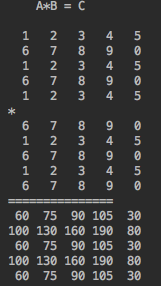
\includegraphics[width=.8\linewidth]{result}
    \caption{Результат работы программы}
    \label{fig:result}
\end{figure}

\section*{Выводы}
В ходе работы были исследованы методы поиска решений задач в пространстве
состояний, а также решения логических задач с применением этих методов.

\end{document}